\documentclass{article}
\usepackage{tikz}
\usetikzlibrary{positioning}  % Added this to enable 'of' positioning
\usepackage{listings}
\usepackage{graphicx}
\lstset{
  basicstyle=\ttfamily\small,
  breaklines=true,
  frame=single
}

\title{RPC File Transfer System}
\author{Your Name}
\date{\today}

\begin{document}

\maketitle

\section{Design of the RPC Service}
The RPC service is designed using Python's built-in \texttt{xmlrpc} library, which allows the client to call remote procedures on the server over HTTP. The server exposes a single method \texttt{get\_file(filename)}, which reads the requested file and returns its binary content wrapped in \texttt{xmlrpc.client.Binary} for safe transmission. The client invokes this method and saves the received data locally.

\begin{figure}[ht]
\centering
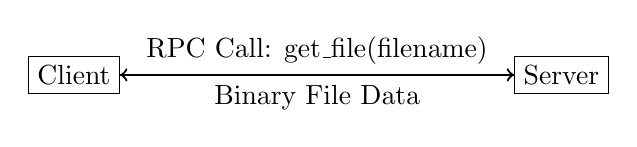
\begin{tikzpicture}
  \node[draw, rectangle] (client) {Client};
  \node[draw, rectangle, right=of client, xshift=4cm] (server) {Server};
  \draw[->, thick] (client) -- node[above] {RPC Call: get\_file(filename)} (server);
  \draw[<-, thick] (client) -- node[below] {Binary File Data} (server);
\end{tikzpicture}
\caption{RPC Service Design}
\label{fig:design}
\end{figure}

\section{Organization of the System}
The system is organized in a new directory called \texttt{RPC}, copied from the original TCP implementation. It contains:
\begin{itemize}
  \item \texttt{server.py}: Manages the RPC server setup and file serving.
  \item \texttt{client.py}: Handles RPC client calls and file saving.
  \item Files to transfer (e.g., \texttt{example.txt}) placed in the server's working directory.
\end{itemize}
No additional subdirectories are needed, as the RPC framework handles communication without raw sockets.

\begin{figure}[h]
\centering
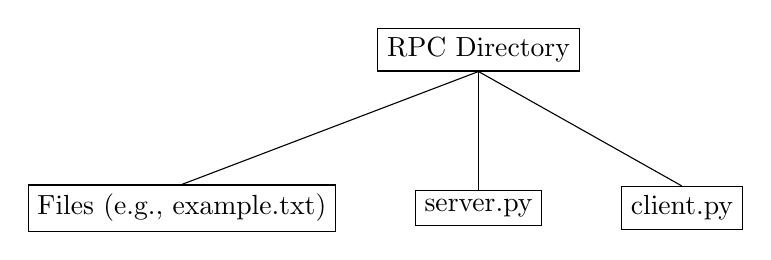
\begin{tikzpicture}
  \node[draw, rectangle] (rpc) {RPC Directory};
  \node[draw, below=of rpc, yshift=-0.5cm] (server) {server.py};
  \node[draw, right=of server] (client) {client.py};
  \node[draw, left=of server] (files) {Files (e.g., example.txt)};
  \draw (rpc.south) -- (server.north);  % Specified anchors to avoid warnings
  \draw (rpc.south) -- (client.north);  % Specified anchors to avoid warnings
  \draw (rpc.south) -- (files.north);   % Specified anchors to avoid warnings
\end{tikzpicture}
\caption{System Organization}
\label{fig:organization}
\end{figure}

\section{Implementation of the File Transfer}
The file transfer is implemented via an RPC method on the server that reads the file and returns it as binary data. The client calls this method and writes the data to a new file. Here is a code snippet from the server:

\begin{lstlisting}[language=Python, caption=Server Code Snippet]
def get_file(self, filename):
    try:
        with open(filename, 'rb') as f:
            return xmlrpc.client.Binary(f.read())
    except FileNotFoundError:
        return xmlrpc.client.Binary(b'File not found')
    except Exception as e:
        return xmlrpc.client.Binary(str(e).encode())
\end{lstlisting}

And from the client:

\begin{lstlisting}[language=Python, caption=Client Code Snippet]
data = proxy.get_file(filename)
if data.data.startswith(b'File not found') or data.data.startswith(b'Error'):
    print(data.data.decode())
else:
    received_filename = f"received_{filename}"
    with open(received_filename, 'wb') as f:
        f.write(data.data)
    print(f"File received and saved as {received_filename}")
\end{lstlisting}

\section{Who Does What}
\begin{itemize}
  \item \textbf{Server}: Listens for RPC requests, reads the requested file from its local filesystem, wraps the content in a binary object, and returns it. Handles errors such as file not found.
  \item \textbf{Client}: Connects to the server via RPC proxy, sends the filename as a parameter, receives the binary data, and saves it to a local file. Checks for error messages in the response.
\end{itemize}

\end{document}